\documentclass[12pt]{extarticle}
\usepackage[utf8]{inputenc}
\usepackage{cite}
\usepackage{graphicx}
\usepackage{float}
\usepackage{amsmath}
\usepackage{hyperref}
\usepackage{enumitem}
\graphicspath{ {images/} }

\setlength{\parindent}{0pt}
\DeclareMathOperator*{\argmax}{argmax} % thin space, limits underneath in displays

\title{Assignment 2}
\author{Ajay Subramanian}
\date{July 2019}

\begin{document}

\maketitle
\setcounter{secnumdepth}{0}

\section{Written Assignment}
\subsection{Question 1}
\begin{enumerate}[label=(\alph*)]
\item TD(0)
	\begin{itemize}
	\item $v(A) = \frac{\frac{3}{5} + \frac{4}{5} + \frac{9}{5}}{3} = \frac{16}{15}$
	\item $v(B) = \frac{3}{5}$
	\item $v(C) = \frac{4}{5}$
	\end{itemize}
	  MC
	\begin{itemize}
	\item $v(A) = \frac{4}{3}$
	\item $v(B) = \frac{3}{5}$
	\item $v(C) = \frac{4}{5}$
	\end{itemize}

\item MDP Diagram
	\begin{figure}[H]
		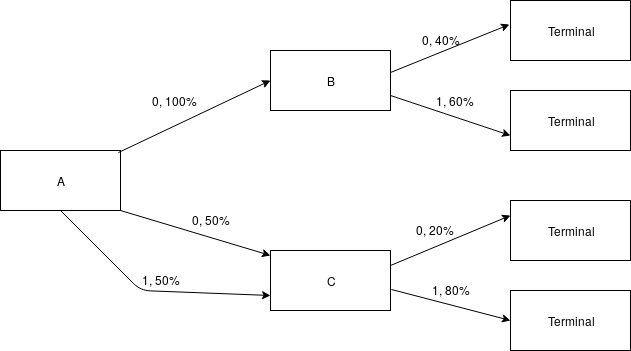
\includegraphics[width=\textwidth, height=10cm]{mdp.png}
		\caption{Markov Decision Process for the given situation}
		\label{fig:mdp}
	\end{figure}
	
\item TD(0)
	\begin{align*}
	\frac{1}{3}\left[2{\left(\frac{16}{15}\right)}^2 + {\left(\frac{1}{15}\right)}^2\right]
	+ \frac{1}{5}\left[3{\left(\frac{2}{5}\right)}^2 + 2{\left(\frac{3}{5}\right)}^2\right]
	+ \frac{1}{5}\left[4{\left(\frac{1}{5}\right)}^2 + {\left(\frac{4}{5}\right)}^2\right] = 1.16
	\end{align*}
	MC
	\begin{align*}
	\frac{1}{3}\left[{\left(\frac{1}{3}\right)}^2 + 2{\left(\frac{4}{3}\right)}^2\right]
	+ \frac{1}{5}\left[3{\left(\frac{2}{5}\right)}^2 + 2{\left(\frac{3}{5}\right)}^2\right]
	+ \frac{1}{5}\left[4{\left(\frac{1}{5}\right)}^2 + {\left(\frac{4}{5}\right)}^2\right] = 1.6222
	\end{align*}
	TD is truer to the training data for this problem since its MSE is lower. For large amoounts of training data, MC will produce a lower MSE than TD(0).

\item TD(0) is truer to the Markov assumption since we use bootstrapping which implicitly creates a dependency between the current state and the next. In MC, the value function is found by averaging returns from multiple sample trajectories. Hence, it will more closely fit the training data.

\item Since the problem is Markovian in nature, TD(0) will produce a lower error on future data. This is because uses the expected reward for updates rather than samples, thereby reducing the chance of updating with outlier reward values.
\end{enumerate}

\subsection{Question 2}
\begin{enumerate}[label=(\alph*)]
\item 
\begin{align*}
G_t =     & (\frac{R_{t+1} + R_{t+2} + ... + R_{t+\tau}}{\beta} + R_{t+\tau+1}) + \\
	       & \gamma(\frac{R_{t+\tau+2} + R_{t+\tau+3} + ... + R_{t+2\tau}}{\beta} + R_{t+2\tau+1}) + \\
	       & {\gamma}^2(\frac{R_{t+2\tau+2} + R_{t+2\tau+3} + ... + R_{t+3\tau}}{\beta} + R_{t+3\tau+1}) + ...\\
	       &; \beta \geq 1, \gamma \leq 1
\end{align*}
It can be observed that this formulation is a modified version of $\tau$-step truncated return.

\item $v_{new}(s) = v(s) + \alpha\left[\frac{R_{t+1} + R_{t+2} + ... + R_{t+\tau}}{\beta} + \gamma v(s_{t+\tau}) - v(s_t)\right]$  
\end{enumerate}

\subsection{Question 3}
\begin{enumerate}[label=(\alph*)]
\item 
\[
E_t(s) = 
\begin{cases}
 max(E_{t-1}(s) - \gamma\lambda,0) & s_t \neq s \\
 E_{t-1}(s) - \gamma\lambda + 1 & s_t = s
\end{cases}
\]

\item 
\[
E_t(s) = 
\begin{cases}
 max(E_{t-1}(s) - \gamma\lambda,0) & s_t \neq s \\
 1 & s_t = s
\end{cases}
\]

\item The linear decay formulation gives importance only to recent states (until $t-\gamma\lambda$) and hence does not waste time on computation for states that temporally occur before that. But in the geometric decay case, the coefficient of all states would be non zero and hence not ideal for large state spaces (would give high variance). Another advantage is that the traces always decrease at the same rate hence making traces of different states more comparable.
\end{enumerate}

\subsection{Question 4}
Using TD(0) in such a case would not be ideal. TD(0) works on the assumption that the next state's value function is solely influenced by the current state and hence holds this state responsible for its performance. This assumption is not true for non-Markovian environments.
One way to solve this issue partially is by using a TD($\lambda$) approach whence varying $\lambda$ between 0 and 1 influences the strength of the Markovian assumption.

\subsection{Question 5}
\begin{alignat*}{3}
  & a \geq 5 &&\rightarrow left && \\
  & a < 5 &&\rightarrow
\begin{cases}
 a \geq 5k & left \\
 a < 5k & right
\end{cases}
\end{alignat*}

\subsection{Question 6}
Episode length = $M.K$ steps\\
Every K steps, the dynamics of the problem change i.e. $P(s',r|s,a)$ changes\\
Problem representation:\\
$s \in S \times M$\\
$a \in A$
$P(s',r|s,a,t//K)$ - Transition probability parameterized by current problem dynamics

\subsection{Question 7}
Yes. Q-learning can be made on-policy by sampling an action from current policy and using the obtained reward in the update, rather than seeking the optimal reward. It will take longer to converge since using the policy for action selection constrains exploration. Using an off-policy method enables us to evaluate using the optimal policy while exploring using the estimation policy.
Yes. We can use importance sampling / weighted importance sampling which use only the ratio of the policy probabilities as a coefficient for the value update equation. This does not require any feedback from the environment/simulation model and hence enables us to compute it off-policy while executing the optimal policy.

\subsection{Question 8}
\begin{enumerate}[label=(\alph*)]
\item 
state set = $\{L, S\}$\\
action set = $\{O\land I, O\land \neg I, \neg O\land \neg I, \neg O\land I\}$\\
Reward and state transition diagram:
\begin{figure}[H]
		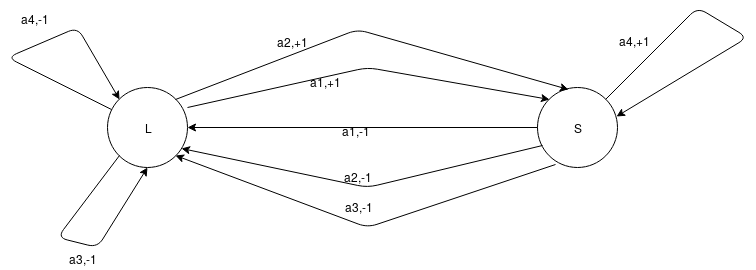
\includegraphics[width=\textwidth, height=7cm]{trans.png}
		\caption{MDP with transitions for the given situation}
		\label{fig:trans}
	\end{figure}

\item 
\textbf{Policy iteration:}\\
	\begin{enumerate}[label=\arabic*)]
	\item 
	\begin{align*}
	v_{\pi}(L) & = -1 + 0.9(0) = -1 \\
	v_{\pi}(S) & = 1 + 0.9(0) = 1 \\
	\pi(L) & = \argmax_a[{1+0.9(1),1+0.9(1),-1+0.9(-1),-1+0.9(-1)}] = a1 \\
	\pi(S) & = \argmax_a[{-1+0.9(-1),-1+0.9(-1),-1+0.9(-1),1+0.9(1)}] = a4 \\
	\end{align*}
	
	\item 
	\begin{align*}
	v_{\pi}(L) & = 1 + 0.9(1) = 1.9 \\
	v_{\pi}(S) & = 1 + 0.9(1) = 1.9 \\
	\pi(L) & = \argmax_a[{1+0.9(1.9),1+0.9(1.9),-1+0.9(1.9),-1+0.9(1.9)}] = a1 \\
	\pi(S) & = \argmax_a[{-1+0.9(1.9),-1+0.9(1.9),-1+0.9(1.9),1+0.9(1.9)}] = a4 \\
	\end{align*}
	\end{enumerate}

\textbf{Value iteration:}\\
	\begin{enumerate}[label=\arabic*)]
	\item
	\begin{align*}
	v(L) = max[1,1,-1,-1] = 1 \\
	v(S) = max[-1,-1,-1,1] = 1
	\end{align*}
	\item
	\begin{align*}
	v(L) = max[1+0.9,1+0.9,-1+0.9,-1+0.9] = 1.9 \\
	v(S) = max[-1+0.9,-1+0.9,-1+0.9,1+0.9] = 1.9
	\end{align*}
	\end{enumerate}
	\begin{align*}
	\pi(L) & = \argmax_a[{1+0.9(1.9),1+0.9(1.9),-1+0.9(1.9),-1+0.9(1.9)}] = a1 \\
	\pi(S) & = \argmax_a[{-1+0.9(1.9),-1+0.9(1.9),-1+0.9(1.9),1+0.9(1.9)}] = a4
	\end{align*}
	
\item Optimal state action values are:\\
L - [2.71,2.71,0.71,0.71]\\
S - [0.71,0.71,0.71,2.71]

\item If you hear laughter, blow organ. If its silent, don't blow the organ and burn incense.
\end{enumerate}

\end{document}